\chapter{Fundamentação teórica}
%\section{Revisão bibliográfica}
Neste capítulo analisou-se a bibliografia existente e executou-se uma revisão em trabalhos correlatos. Nela pesquisou-se sobre arquiteturas de rede disponíveis para utilização durante comunicações de dispositivos IoT, bem como técnicas para aproveitamento de energia disponíveis no ambiente.

%%%%%%%%%%%%%%%%%%%%%%%%%%%%%%%%%%%%%%%%%%%%%%%%%%%%%%%%%%%%%%%%%%%%%%
\section{Low-power wide-area network (LPWAN)} %ch 1303
%%%%%%%%%%%%%%%%%%%%%%%%%%%%%%%%%%%%%%%%%%%%%%%%%%%%%%%%%%%%%%%%%%%%%%
Para dispositivos IoT, um dos objetivos é transmitir dados sem fio usando o mínimo de energia possível. Por isso, os projetistas de aplicações com sensores alimentados por bateria estão particularmente preocupados em enviar dados de sensores de baixa taxa de dados, utilizando comunicação sem fio por quilômetros para minimizar o uso da bateria. Entre as soluções existentes, Bluetooth e Zigbee são projetados para aplicações de curto alcance, já as redes de dados de celular precisam comportar uma quantidade massiva de dados. As redes de baixa potência e grande cobertura (LPWAN) que tornaram-se uma solução popular para este problema. Na Figura~\ref{fig:LPWAN} é possível ver alguns tipos de redes em função do alcance e largura de rede, com destaque especial para as redes LPWAN.


\begin{figure}[h!]
  \caption{Tipos de redes em função do alcance e da largura de banda.}
  \begin{center}
      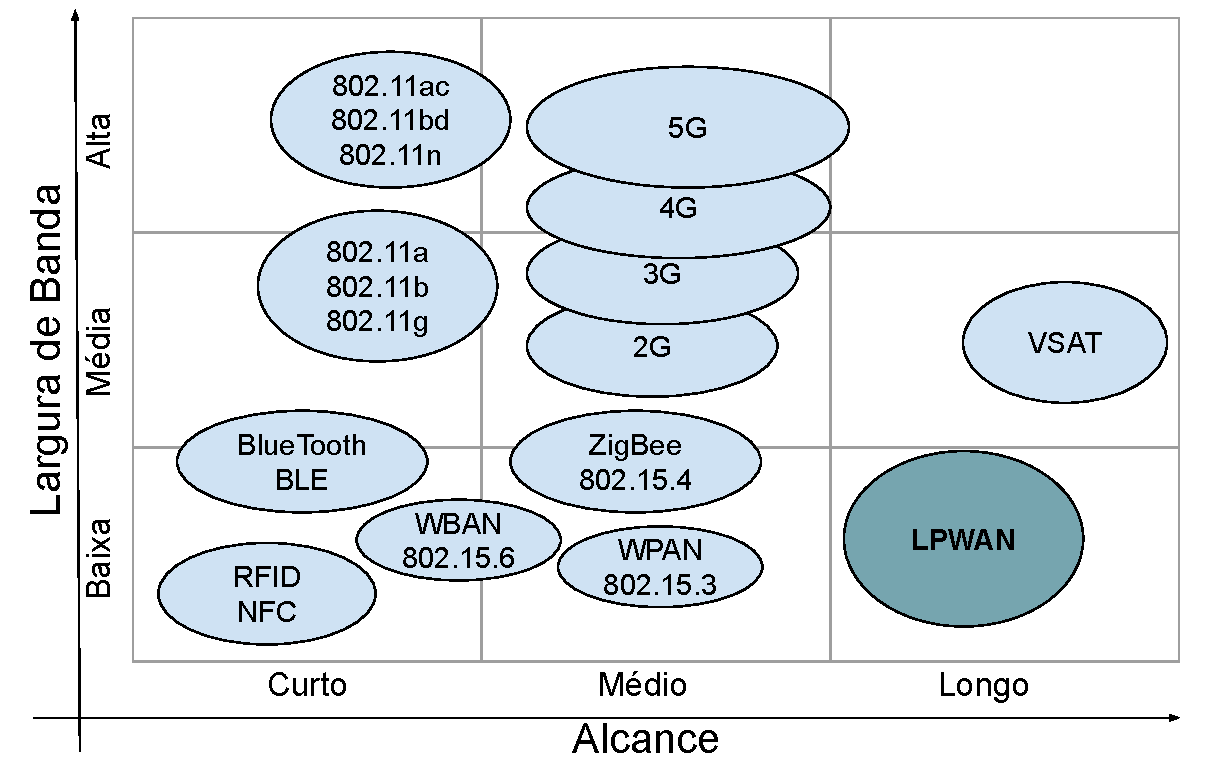
\includegraphics[scale=0.7]{img/LPWAN.pdf}
  \end{center}
  \fonte{Adaptado pelo autor.}
  \label{fig:LPWAN}
\end{figure}
%\Floatbarrier

Redes \textit{LPWAN} tem crescido em volume devido a sua versatilidade em aplicações \textit{IoT} significativamente desde 2017. De acordo com \citeonline{Mane2021}, as duas principais tecnologias que dominam este mercado, \textit{LoRa} e \textit{Sigfox} apresentam resultados de performance compatíveis para esse tipo de aplicação, podendo ainda possuir configurações diferentes de ganhos para cada necessidade.


%%%%%%%%%%%%%%%%%%%%%%%%%%%%%%%%%%%%%%%%%%%%%%%%%%%%%%%%%%%%%%%%%%%%%%
\subsection{LoRa}
LoRa~\cite{LoRaAlliance} é a camada física ou a modulação sem fio utilizada para criar o link de comunicação de longo alcance. Muitos sistemas sem fio legados usam a modulação FSK \textit{(Frequency Shifting Keying}) como a camada física porque é uma modulação muito eficiente para alcançar baixa potência. O LoRa é baseado na modulação de espalhamento espectral, que mantém as mesmas características de baixa potência da modulação FSK, mas aumenta significativamente o alcance da comunicação. 

Esta comunicação é semelhante ao FM, pois modula um sinal alterando sua frequência. No entanto, enquanto um sinal FM muda a frequência instantaneamente, um sinal LoRa aumenta ou diminui a frequência lentamente ao longo de um período de tempo. Esse aumento ou diminuição gradual é chamado de \textit{chirp}, e a taxa de mudança de frequência ao longo do tempo é chamada de \textit{`chirpiness'}. 

O espalhamento espectral tem sido usado em comunicações militares e espaciais por décadas devido às longas distâncias de comunicação que podem ser alcançadas e robustez à interferência, mas o LoRa é a primeira implementação de baixo custo para uso comercial.

As redes LoRaWAN distribuem-se em uma topologia estrela, com protocolos de comunicação e acesso projetados para usar o mínimo de energia e minimizar colisões de sinal de vários terminais. Cada \textit{endpoint} envia seus dados para um \textit{gateway}, que transmite os dados para outra rede, como Ethernet ou Wi-Fi. Os dados recebidos pelo \textit{gateway} são transmitidos pela rede para um computador central que fará o armazenamento ou processamento adicional.
%%%%%%%%%%%%%%%%%%%%%%%%%%%%%%%%%%%%%%%%%%%%%%%%%%%%%%%%%%%%%%%%%%%%%%
\subsection{Sigfox}
%%%%%%%%%%%%%%%%%%%%%%%%%%%%%%%%%%%%%%%%%%%%%%%%%%%%%%%%%%%%%%%%%%%%%%

A Sigfox oferece uma solução de comunicação baseada em software, onde toda a complexidade de rede e computação é gerenciada na nuvem, e não nos dispositivos. Tudo isso junto, reduz drasticamente o consumo de energia e os custos dos dispositivos conectados.


Um dos desafios mais significativos enfrentados pela Internet das Coisas (IoT) é a capacidade de adicionar nós sensores sem fio de maneira fácil e econômica. Sigfox é uma rede proprietária destinada a ouvir bilhões de objetos transmitindo dados, sem a necessidade de estabelecer e manter conexões de rede. O link sem fio precisa ser de baixa potência para que os nós possam funcionar por anos com uma única bateria e ainda ter longo alcance para que milhares de nós possam se conectar ao gateway para coletar dados.

A empresa francesa Sigfox desenvolveu um protocolo de rádio de baixa potência, implementação de rede e infraestrutura de computação em nuvem que pode ser usado para conectar milhões de dispositivos sem fio de baixa potência. Para isso, o protocolo de baixo consumo combinado com uma rede de \textit{gateways} semelhantes a sistemas de telefonia celular, mas que diferentemente de aplicações \textit{machine-to-machine} (M2M) em redes celulares, as redes Sigfox são dedicadas a dispositivos IoT para monitoramento de saúde, energia, temperatura e umidade e até mesmo sensores de segurança.

A rede foi otimizada para longo alcance e baixa potência usando modulação do tipo \textit{differential binary phase shift keying} (DBPSK). Este é um tipo de modulação robusto e altamente eficiente que transporta um bit por símbolo e não precisa de recuperação de portadora. A robustez da codificação permite o longo alcance, e a simplicidade ajuda a manter o consumo de energia baixo, pois pode ser tratado por um processador de 8 bits. Com uma taxa de dados de 100 bits/s é adequada para aplicações de nó de sensor sem fio de longo alcance e baixa potência com atualizações regulares de pequenas quantidades de dados.

%%%%%%%%%%%%%%%%%%%%%%%%%%%%%%%%%%%%%%%%%%%%%%%%%%%%%%%%%%%%%%%%%%%%%%
\subsection{Comparação entre as redes}
%%%%%%%%%%%%%%%%%%%%%%%%%%%%%%%%%%%%%%%%%%%%%%%%%%%%%%%%%%%%%%%%%%%%%%
Redes LoRaWAN e Sigfox, apresentam soluções que podem divergir sobre alguns aspectos, como o fato das redes LoRaWAN necessitarem de uma implementação da infraestrutura de rede com gateway e servidores. Já na rede Sigfox, a infraestrutura de rede é comercializada pela própria empresa, imputando à solução o pagamento de taxas relacionadas à comunicação. O Quadro~\ref{qd:LoraVsSigfox} apresenta uma comparação entra as características técnicas de cada tecnologia.

\begin{quadro}
\caption{Comparação entre LoRa e Sigfox.}
\label{qd:LoraVsSigfox}
  \begin{center}
      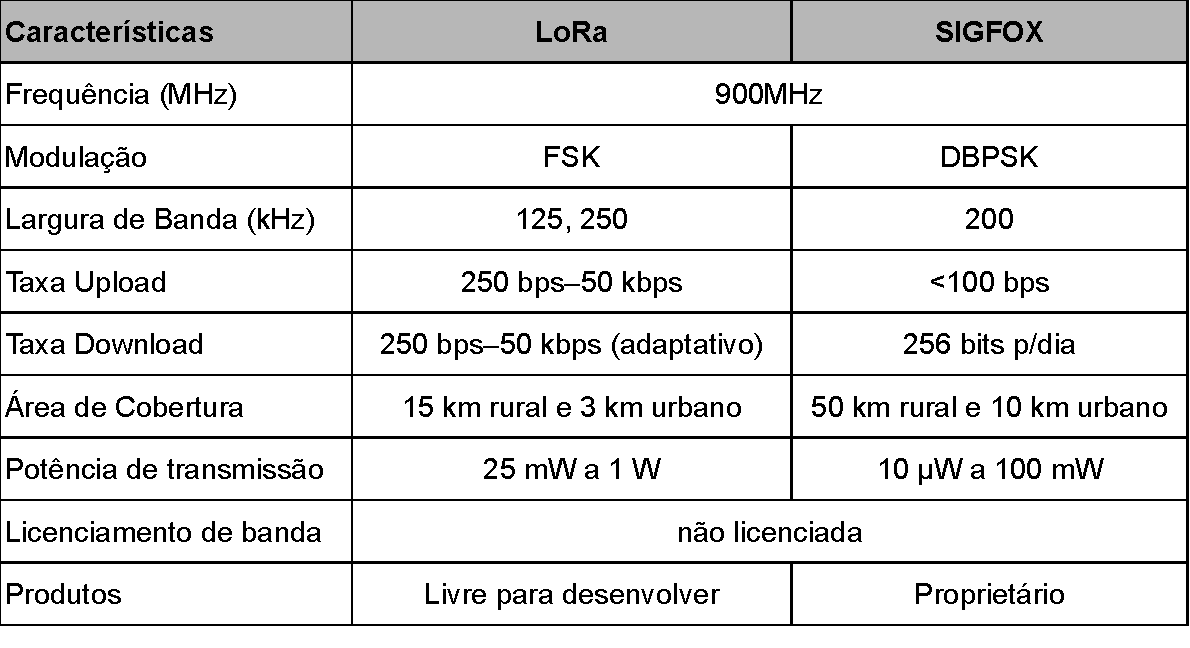
\includegraphics[scale=0.76]{img/LoraVsSigfox.pdf}
  \end{center}
\fonte{Elaborado pelo autor.}
\end{quadro}


%%%%%%%%%%%%%%%%%%%%%%%%%%%%%%%%%%%%%%%%%%%%%%%%%%%%%%%%%%%%%%%%%%%%%%
\section{Energy Harvesting}
%%%%%%%%%%%%%%%%%%%%%%%%%%%%%%%%%%%%%%%%%%%%%%%%%%%%%%%%%%%%%%%%%%%%%%
\textit{Energy Harvesting} (EH) é um termo em inglês que pode ser traduzido como ``Colheita de Energia'' e consiste e coletar energia de algum meio para empregar em um outro uso. Por milênios os seres humanos vêm criando e aperfeiçoando técnicas de coletar energia de um modo cada vez mais eficiente e diversificado.

As técnicas podem variar, mas pode-se coletar energia atualmente com as seguintes fontes: solar, de vibrações, térmica, cinética, piezoelétrica e de radiofrequência. Muitas fontes de energia se consolidaram no último século como a cinética em casos que transforma o movimento dos rios em energia através de usinas hidrelétricas, bem como os painéis solares que transformam a energia solar em eletricidade. Entretanto, estes meios caracterizam-se por converter grandes volumes de energia para abastecer grandes populações. 

Já em sistemas IoT que necessitam de mobilidade, esta tarefa encontra um desafio devido ao espaço que estes capturadores de energia necessitam. Além do mais, devido à mobilidade, nem sempre algumas fontes podem estar presente, como a luz solar, uma vez que este sistema se encontre em um local fechado. 

Nestes casos, a escolha da fonte de energia deve ser analisada respeitando os critérios de disponibilidade da fonte nos locais por onde este dispositivo efetuará o seu deslocamento. Dentre as possibilidades de aproveitamento de energia para sistemas IoT, um deles se destaca por sua crescente disponibilidade. O crescente aumento do número de dispositivos de RF para redes ISM (\textit{Industrial, Scientific and Medical}) aponta para um caminho de alta disponibilidade de potência de sinal disponível nesta banda de frequência. No Brasil, a faixa que compreende as frequências de 902 MHz até 928 MHz alocou-se para este tipo de aplicações. Em um estudo realizado por~\citeonline{manuel}, pode-se obter uma medição da potência de sinal de RF ao logo de uma faixa do espectro de frequências em uma estação de metrô da Inglaterra. Pode-se observar na Figura~\ref{fig:espectro} que nesta mesma faixa citada acima, há uma grande alocação de potência, indicando significativa disponibilidade de energia a ser coletada.

\begin{figure}[h!]
  \caption{Densidade de potência de RF medida fora da estação Northfields London.}
  \begin{center}
      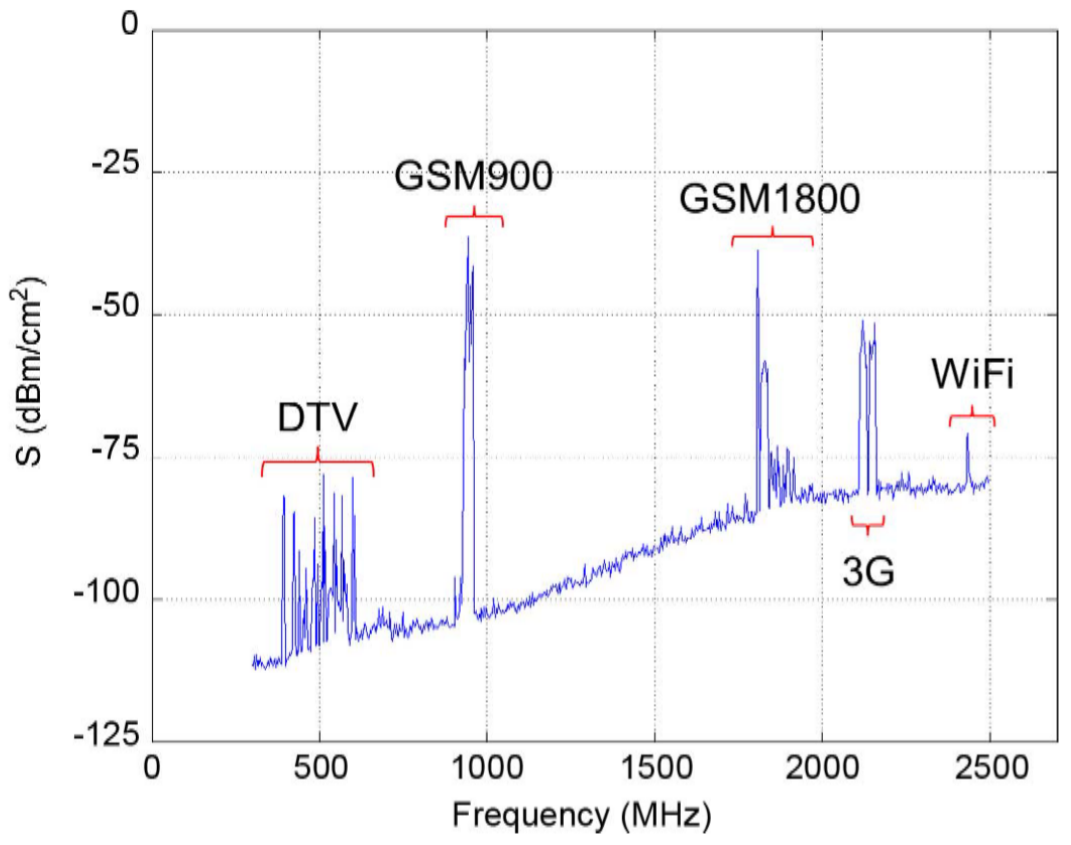
\includegraphics[scale=0.4]{img/espectro.png}
  \end{center}
  \fonte{~\cite{manuel} }
  \label{fig:espectro}
\end{figure}
%\Floatbarrier
%%%%%%%%%%%%%%%%%%%%%%%%%%%%%%%%%%%%%%%%%%%%%%%%%%%%%%%%%%%%%%%%%%%%%%
\section{Wake-up Receiver}
%%%%%%%%%%%%%%%%%%%%%%%%%%%%%%%%%%%%%%%%%%%%%%%%%%%%%%%%%%%%%%%%%%%%%%
Devido à escolha por um sistema sem baterias, algumas contensões precisam ser executadas para a operação do sistema de forma a desperdiçar o mínimo de energia. Embora o monitoramento de temperaturas de operação implique em um custo energético, o mesmo em nada se compara a uma transmissão de rádio, ou até mesmo a manutenção de uma recepção de rádio por longos períodos de tempo. Por isso se faz necessário um mecanismo responsável por ligar o receptor para aguardar uma comunicação. Neste cenário, o custo energético se mantém apenas por um intervalo curto de tempo. Mas para identificar o início dessa comunicação, utiliza-se o método chamada \textit{Wake-up Receiver}. 

Com base nisso, \citeonline{ferreira} classifica como vantajosa a utilização de um circuito receptor adicional de baixa potência operando como um gatilho para o receptor principal. Com a identificação deste sinal, um microcontrolador pode ser acordado por interrupção e executar a inicialização do receptor principal.

Uma vez que o sistema esteja acordado, ele pode inclusive realizar uma medição da energia armazenada no sistema de coleta para decidir pelo ligamento do receptor ou não. Uma vez que o sistema identifique as condições propícias para o receptor de rádio principal, este pode aguardar pelos comandos básicos e após um tempo o sistema volta a dormir em modo profundo de consumo de energia.

Para desenvolvimento e aplicação deste circuito, usou-se como referência conceitual o circuito integrado desenvolvido pelo \textit{Fraunhofer Institute Integrated Circuits and Systems} de acordo com o Anexo~\ref{ax:wake}, que apresenta sensibilidade de -80~dBm e um consumo de corrente inferior a 3~$\mu$A @ 1,8~V.

%%%%%%%%%%%%%%%%%%%%%%%%%%%%%%%%%%%%%%%%%%%%%%%%%%%%%%%%%%%%%%%%%%%%%%
\section{Trabalhos correlatos}

Todos os trabalhos mencionados no Quadro~\ref{qd:correlatos} possuem as suas particularidades de aplicação à projetos que envolvem a análise ou monitoramento de redes inteligentes de distribuição de produtos perecíveis. Não necessariamente envolvendo alimentos, ou especificamente o monitoramento, mas traçando algum paralelo com o presente trabalho.
Alguns dos trabalhos são mais superficiais, outros mais profundos, porém todos demonstram alinhamento com o tema proposto.

\begin{quadro}
  \caption{Trabalhos Correlatos.}
  \begin{center}
      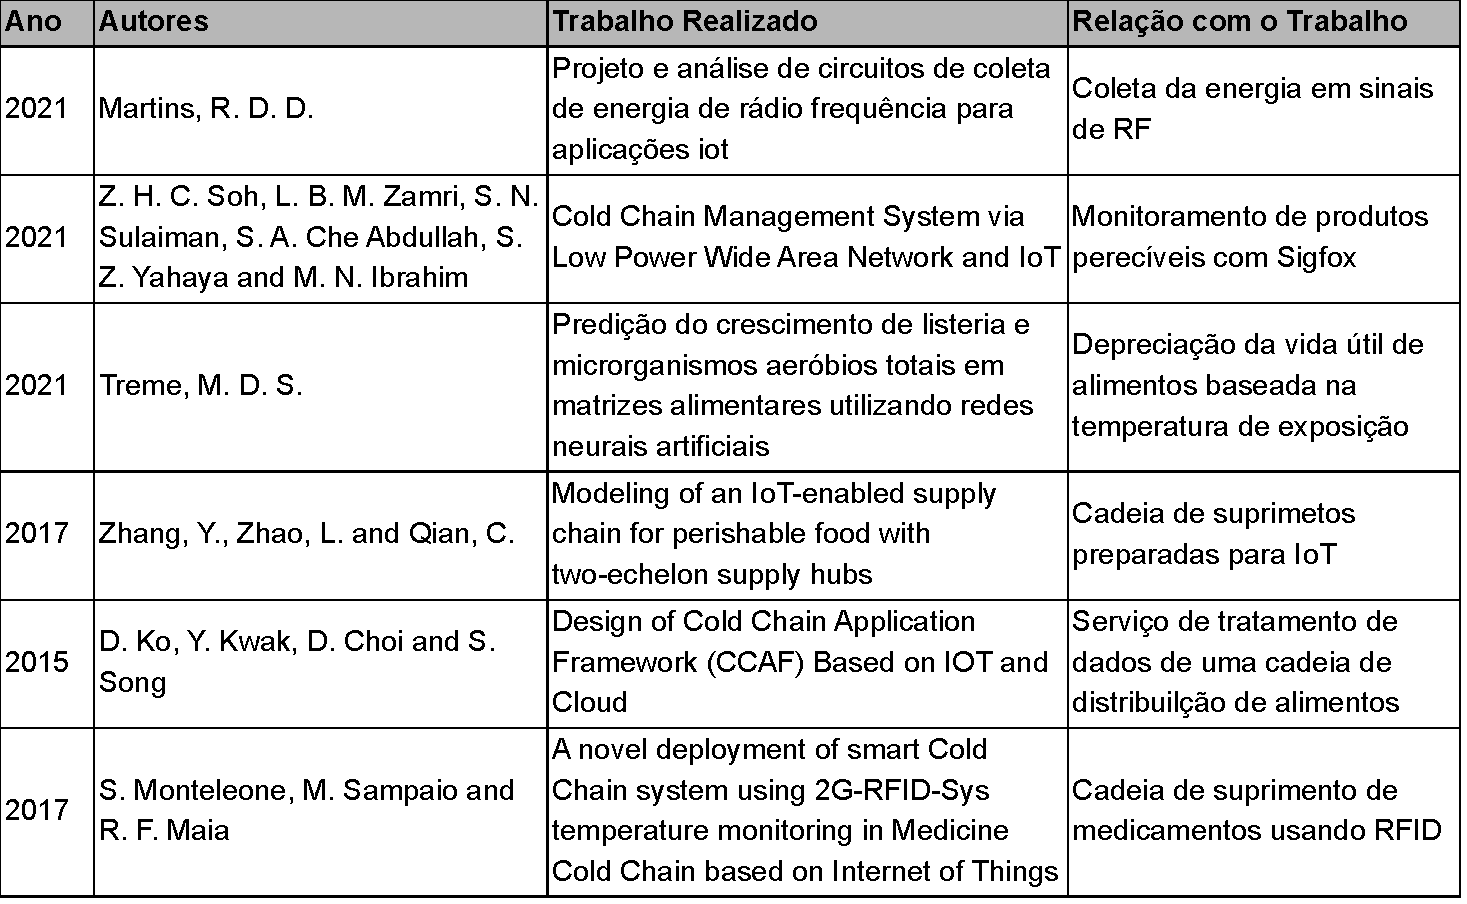
\includegraphics[scale=0.64]{img/correlatos.pdf}
  \end{center}
  \fonte{Elaborado pelo autor.}
  \label{qd:correlatos}
\end{quadro}

No trabalho de~\citeonline{renan}, é feita uma avaliação sobre o desenvolvimento de um chip para colheita de energia por RF. Esse estudo ainda apresenta em sua conclusão uma sugestão para a criação de um dispositivo IoT alimentado por capacitor.

Já~\citeonline{Soh}, aborda uma questão muito relevante sobre as exigências internacionais no transporte de produtos perecíveis que carecem de uma temperatura controlada. Como solução a isso é empregado uma solução de IoT utilizando a rede Sigfox para acompanhamento dos dados em tempo real.

Tratando da questão biológica do crescimento bacteriano em alimentos perecíveis~\citeonline{monica} além de discorrer sobre o tema e analisar o perfil de crescimento bacteriano, propõe uma solução para estimar a data de validade desse alimentos a partir do perfil de temperatura a que esses alimentos foram expostos utilizando redes neurais artificiais.

Para~\citeonline{Zhang2017}, a importância de colocar um olhar sobre a cadeia de distribuição logística de alimentos perecíveis. Considerando para isso os pontos de distribuição intermediários onde se faz tanto o manejo de cargas, como a possibilidade de verificação do estado atual do ciclo. Embora nesse trabalho haja uma busca pela padronização de um sistema IoT específico para alimentos perecíveis analisando a cadeia de distribuição presente na China, pode-se comparar com o trabalho executado por~\citeonline{Aliotte2022} que faz uma análise da cadeia de distribuição no Brasil.

Na pesquisa de~\citeonline{Ko2016} está apresentado uma solução para gerenciamento de produtos perecíveis dentro de uma rede de distribuição. Nesse caso, a inteligência do sistema se dá em função da organização e alocação destes alimentos em câmaras frigoríficas de modo a evitar que algum alimento fique armazenado por muito tempo. Embora esse trabalho seja voltado para armazenamento, pode-se notar que o problema de logística não está relacionado apenas ao transporte, mas também na armazenagem dos mesmos.

Em uma última análise~\citeonline{Monteleone2017} apresenta soluções de governança para a cadeia de suprimento de medicamentos que podem ser em tempo real ou não. Para isso é apresentada uma solução baseada em RF-ID para esse acompanhamento e controle, sendo possível uma responsabilização de qualquer prejuízo a partir dos dados de controle do processo de logística. Esse estudo mostra as possibilidades de uso dos dados coletados em campo não só para o entendimento do processo de transporte, mas mostra um caminho para o aumento da qualidade das redes de transporte para produtos desse tipo.


%%%%%%%%%%%%%%%%%%%%%%%%%%%%%%%%%%%%%%%%%%%%%%%%%%%%%%%%%%%%%%%%%%%%%%

